%%%%%%%%%%%%%%%%%%%%%%%%%%%%%%%%%%%%%%%%%%%%%%%%%%%%%%%%%%%%%%%%%%%%%%
% 
% Model copied by overleaf.
%
%%%%%%%%%%%%%%%%%%%%%%%%%%%%%%%%%%%%%%%%%%%%%%%%%%%%%%%%%%%%%%%%%%%%%%

\documentclass[12pt]{article}

\usepackage{sbc-template}

\usepackage{graphicx,url}

%\usepackage[brazil]{babel}   
\usepackage[utf8]{inputenc}  

     
\sloppy

\title{ZeroMQ Distributed Message Middleware\\Uma breve abordagem}

\author{Eduardo Pedersetti José\inst{1}, Ivan Andreis\inst{1}, Leonardo S. Paula\inst{1}}

\address{Ciência da Computação -- Universidade do Vale do Rio dos Sinos (UNISINOS)\\
  Caixa Postal 15.064 -- São Leopoldo -- RS -- Brasil
\email{\{eduardoxy,ivann.andreis,leonardopaula\}@gmail.com}
}

\begin{document} 

\maketitle

\begin{abstract}
  This paper aims to bring an overview about ZeroMQ middleware. This concurrency framework written in C++, has high performance, and is focused in sending asynchronous messages, being used in distributed systems applications, and providing all the necessary tools for the developers that want to create their own message queue systems.
\end{abstract}
     
\begin{resumo} 
   Este artigo tem como objetivo trazer uma visão geral sobre o middleware ZeroMQ. Este framework de concorrência escrito em C++ e de alta performance, com foco no envio de mensagens assíncronas, é utilizado em aplicações de sistemas distribuídos, fornecendo ao desenvolvedor todas a ferramentas necessárias para criar seu próprio sistema de fila de mensagens.
\end{resumo}

\section{Middleware}
	A evolução das redes de computadores com o advento da internet facilitaram a ploriferação de aplicações distribuídas. Sabendo que as partes interessadas de uma aplicação distribuída podem executar em diferentes locais físicos, diversas vantagens podem ser adicionadas à aplicações distribuídas, como tolerância a falhas (através de replicação) e aumento de performance, através da paralelização de tarefas, por exemplo.

	Analisando ambientes onde os Sistemas Distribuídos são executados, nota-se uma heterogeneidade entre os dispositivos que estão se comunicando. Podem existir, em um mesmo Sistema Distribuído, diferentes plataformas de hardware, tecnologias de rede, sistemas operacionais e linguagens de programação. Essas particularidades podem tornar o desenvolvimento de um SD um grande desafio  (Extraído do Livro Distributed Systems Architecture).

	É notável, portanto, que para propiciar o desenvolvimento de uma aplicação distribuida, faz-se necessária uma infraestrutura adequada, que permita o desenvolvimento e execução de um SD. Essa infraestrutura necessária é fornecida por um middleware. Um middleware é uma camada de software que reside entre a aplicação e a API de acesso à rede, sendo responsável por abstrair os detalhes de rede que podem ser ignorados pela aplicação (conforme ilustrado na Figura~\ref{fig:fig_middleware}).

	A rede simplesmente fornece o acesso à camada de transporte, e seu acesso difere dependendo da tecnologia e da plataforma física utilizadas. O Middleware homogeniza o acesso às redes, oferecendo serviços genéricos às aplicações. Além de interligar diferentes domínios de tecnologias e encapsular as diferenças entre os sistemas. (Extraído do Livro Distributed Systems Architecture) Como o middleware é uma interface entre a API de acesso à rede e a aplicação, ele possui duas visões: a visão do programador da aplicação e a visão do programador do sistema.

% Imagem da ilustração de um middleware.
\begin{figure}[ht]
\centering
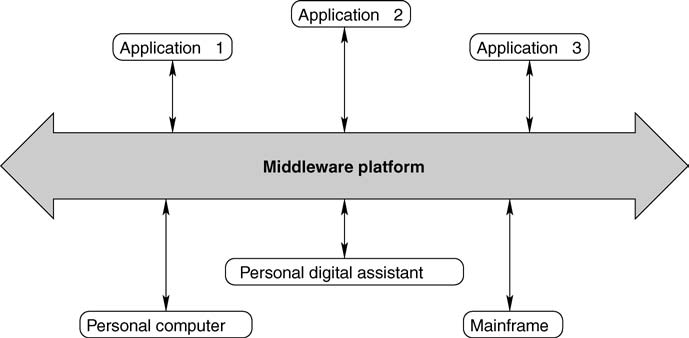
\includegraphics[width=.5\textwidth]{Img_Middleware_Arc.png}
\caption{Arquitetura básica de um middleware}
\label{fig:fig_middleware}
\end{figure}

	O programador da aplicação vê o Middleware como uma ferramenta de auxílio para o desenvolvimento de aplicações distribuídas. Estes programadores não estão interessados em como que o Middleware é implementado, mas sim em como obter acesso prático aos seus recursos. O Middleware é uma caixa-preta para o programador da aplicação, com uma interface de acesso bem definida.

	O programador de sistemas vai além. Para ele o Middleware é uma caixa-branca, e seu interesse maior não está em como esta caixa interage com o mundo externo, mas sim em como ocorrem os seus processos internos. A aplicação que utilizará o Middleware, para o programador de sistemas, tem uma importância menor. O ponto de referência comum à ambos, programador de sistema e de aplicações, é a interface fornecida pelo middleware que será utilizada pelas aplicações.

\section{Filas de Mensagens}
	Filas de Mensagens, ou message queues, são conhecidas tecnicamente como FIFO (First In First Out). Consistem em uma estrutura de dados bem definida e estudada. Diferentes formas de implementação de FIFO, como filas de prioridades e filas duplamente terminadas (deque - Double End Queue), já estão consolidadas na implementação de algoritmos para troca de dados. A ideia de uma fila de mensagens é simples: a informação é armazenada na fila e é buscada quando estiver pronta ou quando o requisitante da informação à solicitar.

	Embora a ideia seja simples, a sua implementação nem sempre é trivial. Para implementar uma fila de mensagens simples em memória, alguns problemas podem surgir, como quedas de energia elétrica ou falhas de hardware, e o conteúdo inteiro da fila será perdido. Quando isso ocorre, o programa que está à espera de uma mensagem da fila corrompida não receberá nenhuma mensagem.

	Para contornar este e outros problemas, utilizamos dispositivos que implementam filas de mensagens. Na Figura~\ref{fig:fig_msgqueue} há uma ilustração da arquitetura básica de uma fila de mensagens. Ao adotar um dispositivo que gerencia uma fila de mensagem, se tem uma garantia à priori de que todas as mensagens serão entregues ao seu destinatário, independentemente do que aconteça. As filas de mensagens tem um papel importantíssimo em Sistemas Distribuídos: habilitar a comunicação assíncrona de processos.

\begin{figure}[ht]
\centering
	
\includegraphics[width=.85\textwidth]{Img_MsgQueue.png}
\caption{Arquitetura Fila de Mensagens}
\label{fig:fig_msgqueue}
\end{figure}

	Em vez de utilizar um componente que implemente uma fila de mensagens, podem ser utilizadas outras abordagens, como uma thread que gerencia uma fila de mensagens ou até diversas threads para gerenciar uma única fila. Porém estas abordagens trazem alguns pontos negativos. Em um sistema single-thread, a aplicação pode não ser capaz de processar todas as requisições quando o número de clientes for muito grande. Em um sistema multi-thread, a aplicação pode ficar vulnerável à um ataque de negação de serviço (Distributed Denial of Service - DDoS). Além disso, todas as informações da fila poderão ser perdidas no caso de falta de energia ou falha de  hardware, por exemplo. Portanto, a utilização de um sistema de fila de mensagens confiável é imprescindível para a execução de um sistema distribuído.

\section{ZeroMQ} \label{sec:firstpage}
	O ZeroMQ é um software opensource apoiado por uma comunidade ativa e com suporte comercial pago. Ele fornece ferramentas para construção de arquiteturas centralizadas, distribuídas, pequenas ou grandes. Pode transmitir as mensagens através de IPC, TCP, TIPC e multicast. O ZeroMQ fornece padrões como publish-subscriber, push-pull, e router-dealer, além de mecanismos de entrada e saída de alta velocidade.

	A definição formal do ZeroMQ é a seguinte: o ZeroMQ é uma biblioteca de mensagem feita para ajudar os desenvolvedores a projetarem aplicações distribuídas e concorrentes. Embora o ZeroMQ, conhecido também como ZMQ, seja similar à uma fila de mensagens (ou message queue), é importante enfatizar que este não é um sistema de fila como o ActiveMQ, WebSphereMQ ou RabbitMQ. O ZMQ fornece todas as ferramentas necessárias para que o desenvolvedor desenvolva o seu próprio sistema de fila de mensagens, ou seja, o ZMQ é uma biblioteca, desenvolvida nativamente na linguagem C e podendo ser utilizada em diversas plataformas. Atualmente, o ZMQ oferece suporte a mais de vinte linguagens de programação, entre elas C/C++, Ruby, PHP, Python, Node.js, entre outras.

	O ZMQ é uma biblioteca simples. Operações de IO assíncronas podem enfileirar mensagens em uma thread para tratamento de entradas e saídas. Estas threads trabalham de maneira assíncronas ao tratar o fluxo da rede, deixando o restante do trabalho a ser realizado pelo próprio desenvolvedor. O ZMQ oferece uma interface simplificada para o trabalho com sockets se comparada às diretivas utilizadas na linguagem C, por exemplo.

\subsection{Histórico}
	Pieter Hintjens, atual CEO da iMatix, iniciou o projeto do ZeroMQ juntamente com Martin Sustrik, vindo a registrar o domínio zeromq.org em maio de 2007. Martin foi o arquiteto de software e líder de desenvolvimento do projeto até o final de 2011. 

	Como ponto alto de reconhecimento da performance do ZMQ, podemos citar o CERN(Conseil Européen pour la Recherche Nucléaire), acelerador de partículas, que em 2011 fez um levantamento buscando formas de unificar soluções de middleware usadas para operar seus aceleradores. o ZMQ concorreu com middlewares como CORBA, Ice, Thrift, YAMI4, RTI and Qpid, em um estudo que comparou duas implementações open source, ganhando dos seus concorrentes muito devido a sua versatilidade, incluindo a fácil adaptação ao LynxOS.

	Outra versão, chamada JeroMQ, foi anunciada em 2012 como a versão pura em JAVA do ZMQ, que inspirou portas nativas para o mesmo, tendo o NetMQ como exemplo. Já em 2013, seu criador e CEO Hintjens, anunciou um novo desenvolvimento do protocolo ZMTP, trazendo inovações em termos de mecanismos de segurança extensíveis para o ZMQ. Por fim, Martin Hurton(not Sustrik), implementou o CurveZMQ posteriormente, um mecanismo de encriptamento e autenticação adicional para a biblioteca principal do ZMQ.

\subsection{Operação/Tecnologia}
	A API do ZMQ provê sockets que são responsáveis pelas conexões muitos-para-muitos entre os pontos. Além disso, o ZQM obriga o uso de um padrão de mensagens, e é otimizado para o seu funcionamento de acordo com o padrão previamente definido. Os padrões básicos existentes são:

	Push-pull: Padrão de coleção de distribuição de tarefas paralelas, conectando nós que podem ter múltiplos passos e loops. Publish-subscribe: padrão de distribuição de dados simples, conectando publishers(publicadores) com subscribers(assinantes). Request-reply: outro padrão de distribuição de tarefas, trata-se de uma chamada de procedimento remoto, conectando um número variado de clientes a um número variado de servidores. Exclusive pair: usado somente em casos específicos, este padrão avançado conecta 2 sockets diferentes em um mesmo par.

	Estes padrões definem topologias de redes particulares, sendo que todos são designados de forma a serem infinitamente escaláveis. O publish-suscribe define a topologia de "árvore de distribuição de dados", enquanto o push-pull utiliza a de "pipeline paralelizada" e o request-reply a de "service bus". As mensagens que passam pelos sockets são tratados como blocos binários de dados. Como já comentado anteriormente, transportes de mensagens disponíveis no ZMQ podem ser feitos através do TCP, PGM(multicast), IPC(Inter-process communication) e ITC(inter-thread communication). O método de transporte via TCP costuma ser o mais escolhido, obtendo boa performance e robustez. Porém, quando não há necessidade de atravessar grandes distâncias via rede, os protocolos IPC e ITC podem obter ganhos ainda maiores em termos de latência. 
    
	O ZMQ implementa um protocolo chamado ZeroMQ Message Transfer Protocol(ZMTP), que define regras de interoperabilidade, mecanismos de segurança extensíveis, e outras funcionalidades a nível de transporte.

	Quanto à sua alta performance, esta ocorre pois a biblioteca interna do ZMQ trabalha com um modelo de threads, podendo superar aplicações TCP convencionais. Além disto, não possui o overhead comum de outros protocolos, como o AMQP, e pode fazer uso de transportes eficientes através de Multicast ou Inter-process communication. Também utiliza conexões de TCP/IP de maneira eficiente, minimizando o overhead no protocolo e nas chamadas de sistemas, graças ao uso de agrupamento para o envio de mensagens de forma inteligente.

	Ao fazer uso do agrupamento de mensagens, o ZMQ evita um número extenso e custoso de operações, garantindo um bom desempenho. Este agrupamento pode ser feito de duas maneiras. Numa delas, o remetente apenas faz o envio das mensagens agrupadas depois que um certo número limite ou limite de tempo é atingido. Na outra, o recebedor das mensagens faz a leitura de todas as mensagens disponíveis em um agrupamento independentemente do número de mensagens disponíveis, podem ter tanto 1 quanto 100 mensagens neste, por exemplo. Ao optar pela última, é possível garantir também uma menor latência, já que as mensagens são lidas instantâneamente assim que o recebedor está disponível para processá-las. Já a primeira, atrasa o envio das mensagens até que o limite pré-definido seja atingido.
    
% Imagem da ilustração batching
\begin{figure}[ht]
\centering
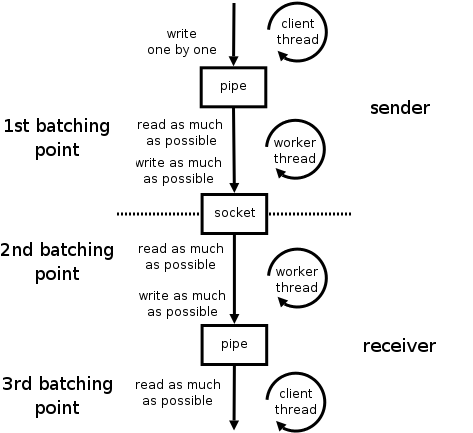
\includegraphics[width=.5\textwidth]{batching.png}
\caption{Exemplo batching}
\label{fig:exampleFig4}
\end{figure}


\subsection{Infraestrutura}

	Uma vez decidida a forma de transporte, faz-se necessário definir também como os componentes irão se conectar uns aos outros. Basicamente, procura-se vincular a parte mais estável da rede a uma porta específica, enquanto as partes mais dinâmicas irão se comunicar a esta. Também é possível que as 2 pontas da rede sejam dinâmicas, dificultando a escolha de um ponto de conexão único. Para estes tipos de casos, o ZMQ proporciona alguma dispositivos de "forwarding" que podem se vincular a duas portas diferentes e encaminhar as mensagens de um para o outro. Desta forma, o dispositivo de encaminhamento se torna o ponto estável da rede, ao qual cada componente pode se conectar.

	Há três tipos diferentes de dispositivos de forwarding fornecidos pelo ZMQ:
	QUEUE: utilizado no padrão de mensagem Request/response;
	FORWARDER: utilizado no padrão de mensagem Publish/subscribe;
	STREAMER: utilizado no padrão de mensagem pipeline.

	Na figura abaixo podemos ver um exemplo simples de um Forwarder, atuando como vinculador de duas portas diferentes, desta forma inicializando a conexão entre o cliente e o servidor e eliminando a necessidade de uma lógica de aplicação adicional, ao manter uma lista dos clientes conectados.

% Uso de forwarding no ZMQ
\begin{figure}[ht]
\centering
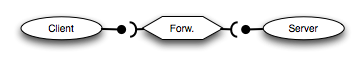
\includegraphics[width=.5\textwidth]{cfs.png}
\caption{Exemplo de uso de um forwarder}
\label{fig:exampleFig3}
\end{figure}

\section{Concorrentes}
	Texto Concorrentes.

\section{Análise}
	Texto análise.

\section{Conclusão}

	Com o avanço da computação móvel, Big Data, IoT(Internet of Things), etc. torna-se cada vez mais crucial o avanço das tecnologias relacionadas à sistemas distribuídos, para que todo esse montante de dados possa ser processado, analisado e utilizado com a maior performance e segurança possíveis. Com isso, os desenvolvedores que atuam no mercado irão se deparar cada vez mais, até mesmo de forma diária, com situações nas quais precisam optar e resolver problemas relacionados aos SDs. Faz-se necessário que este processo seja também de um aprendizado rápido e prático, e o ZeroMQ pode ajudar muito nesta questão, facilitando a vida do desenvolvedor. Este artigo buscou então trazer uma visão geral de um dos middlewares opensource em uso no mercado atual, demonstrando assim as principais características e funcionamento da biblioteca do mesmo, afim de demonstrar sua utilidade.

\section{References}

http://zeromq.org/
http://www.aosabook.org/en/zeromq.html
http://nichol.as/zeromq-an-introduction
https://www.digitalocean.com/community/tutorials/how-to-work-with-the-zeromq-messaging-library

Bibliographic references must be unambiguous and uniform.  We recommend giving
the author names references in brackets, e.g. \cite{knuth:84},
\cite{boulic:91}, and \cite{smith:99}.

The references must be listed using 12 point font size, with 6 points of space
before each reference. The first line of each reference should not be
indented, while the subsequent should be indented by 0.5 cm.

\bibliographystyle{sbc}
\bibliography{sbc-template}

\end{document}
